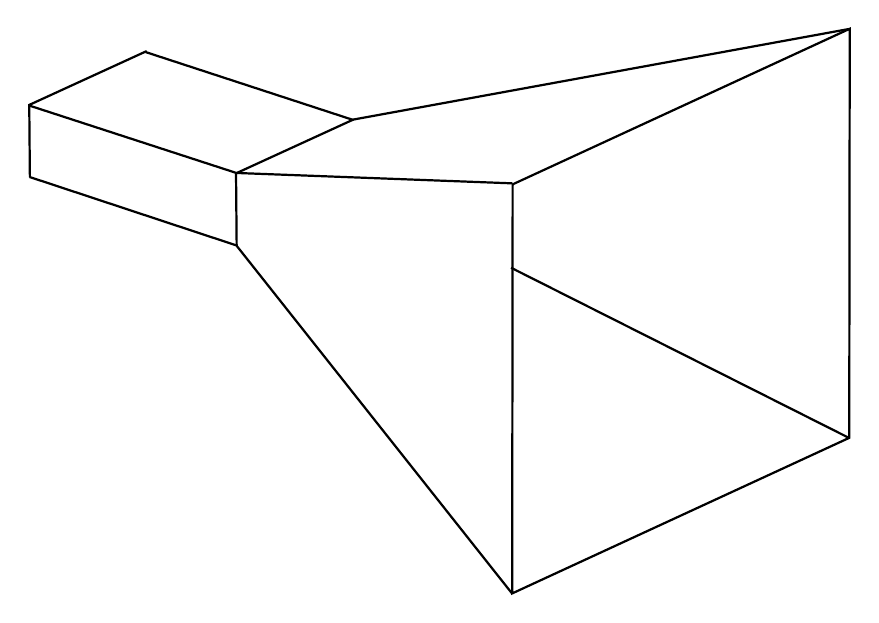
\begin{tikzpicture}

  % Hornöffnung
  \draw[thick]
    (6.179,5.235) --
    (10.460,7.211) --
    (10.454,2.016) --
    (6.173,0.040) --
    cycle;

  % Hohlleiter / Übergang
  \draw[thick]
    (2.674,4.455) --
    (2.666,5.375) --
    (4.158,6.059);

  \draw[thick]
    (0.048,5.324) --
    (0.040,6.244) --
    (1.532,6.928);

  % obere Kanten
  \draw[thick]
    (1.519,6.915) --
    (4.145,6.056) --
    (10.449,7.208);

  % untere Hornkante
  \draw[thick]
    (6.159,4.176) --
    (10.449,2.016);

  % mittlere Hohlleiter- und Hornkante
  \draw[thick]
    (0.034,6.238) --
    (2.670,5.380) --
    (6.176,5.248);

  % untere Kante
  \draw[thick]
    (0.044,5.329) --
    (2.670,4.460) --
    (6.166,0.046);

\end{tikzpicture}